\subsubsection{Pohađanje praktične obuke}

\vspace{3mm}

\begin{itemize}

\item \textbf{Kratak opis:} Kandidat sa instruktorom dogovara časove vožnje. Neophodno je da kandidat prisustvuje ukupno 40 časova i prisustvo se belezi u sistem.

\vspace{2mm}

\item \textbf{Učesnici} \newline
   - Kandidat - korisnik sistema koji pohađa praktičnu obuku.\newline   
   - Instruktor - korisnik sistema koji drži praktičnu obuku. 
   
\item \textbf{Preduslovi:} \newline
   - Sistem je u funkciji. \newline
   - Kandidat je prijavljen za praktičnu obuku 

\item \textbf{Postuslovi:} \newline
    - Kandidat je završio praktičnu obuku.

\item \textbf{Osnovni tok:}  
   \begin{enumerate}
   \item Kandidat otvara formular za zakazivanje časa.
   \item Sistem prijazuje formular.
   \item Kandidat zakazuje čas.
   \item Instruktor potvrđuje čas.
   \item Kandidat prisustvuje času u odgovarajućem terminu.
   \item Instruktor otvara formular za evidenciju časa.
   \item Sistem prikazuje formular.
   \item Instruktor unosi podatke o održanom času.
   \item Kandidat potvrđuje podatke o održanom času.
   \item Sistem čuva unete podatke. \newline
   \end{enumerate}

\item \textbf{Alternativni tok:}  
   \begin{itemize}
   \item A1. \textbf{Kandidat otkazuje čas:}
  Kandidat obaveštava instruktora da ne može da prisustvuje času i zakazuje novi termin časa, proces se nastavlja u koraku 1 osnovnog toka.
   \end{itemize}

\item \textbf{Dodatne informacije:}    
\begin{itemize}
\item Osnovni tok se ponavlja 40 puta. Nakon toga, sistem šalje mejl kandidatu sa potvrdom o žavršenoj praktičnoj obuci.
\end{itemize}

\end{itemize}

\begin{figure}[H]
  \begin{center}
      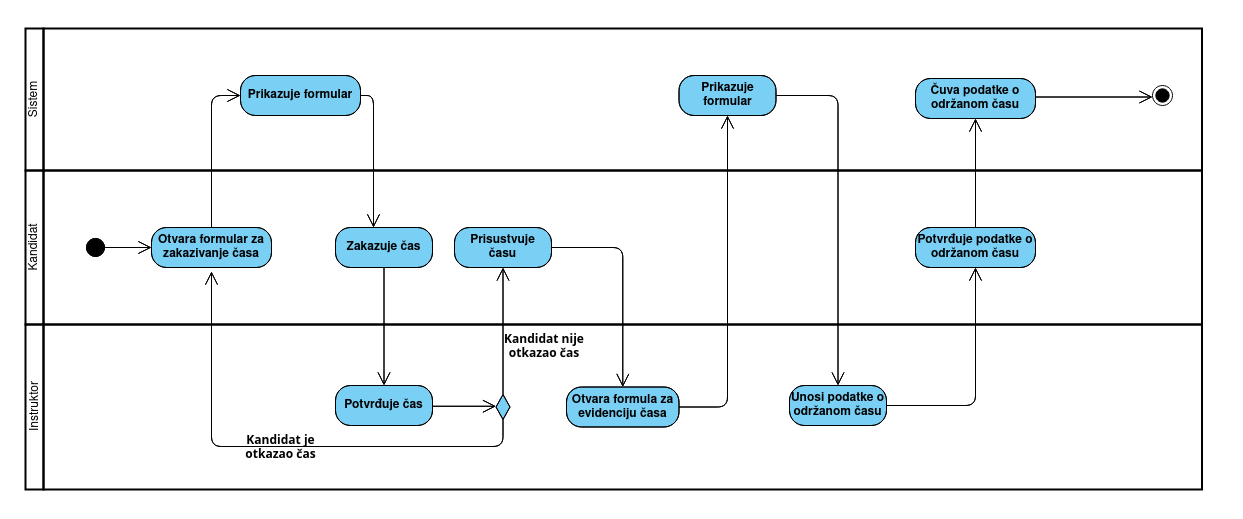
\includegraphics[width=170mm, height=70mm]{Diagrams/dijagram_aktivnosti_pohadjanje_prakticne_obuke.png}
  \end{center}
  \caption {Dijagram aktivnosti - Pohađanje praktične obuke}
  \label{activity_pohadjanje_prakticne_obuke}

\end{figure}
